\begin{figure}[ht]
	\centering
	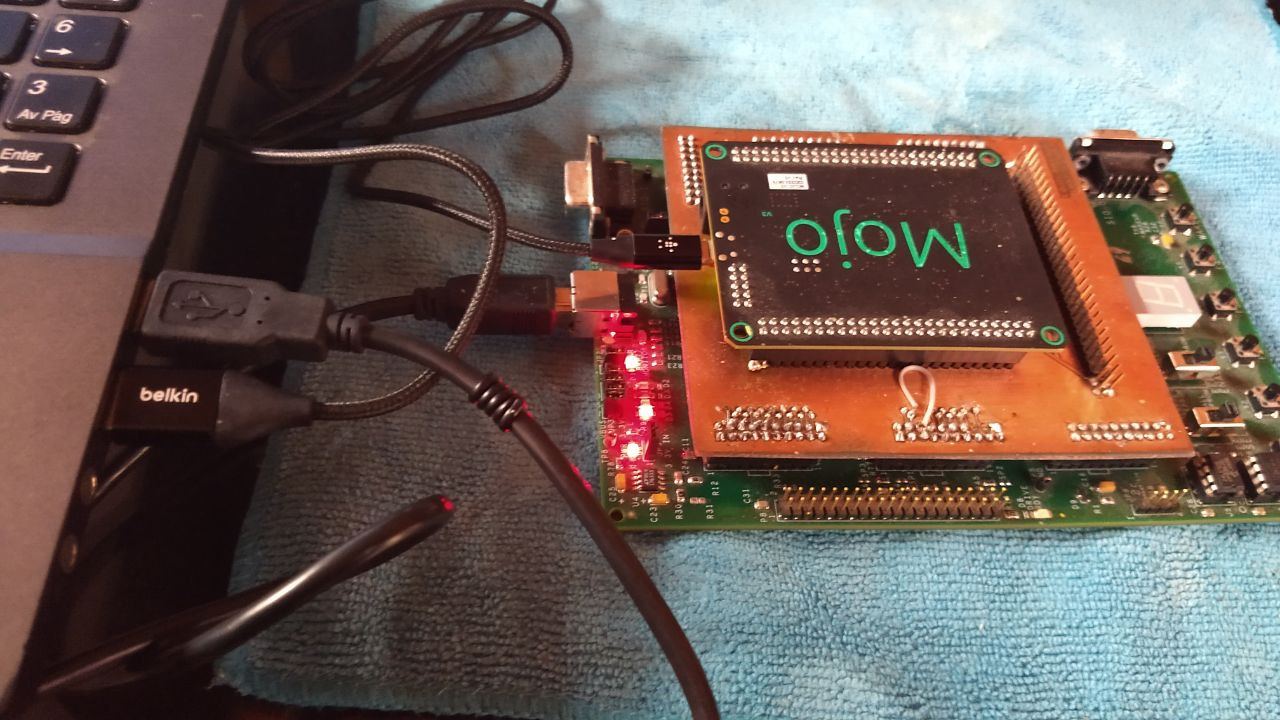
\includegraphics[width=0.7\textwidth]{sistema2.jpg}
	\caption{El sistema desarrollado en funcionamiento}
	\label{test:todo}
\end{figure}

Como se muestra en la Figura \ref{test:todo}, en el sistema completo, montado y en funcionamiento, el FPGA es conectado a la interfaz USB través de la Placa de Interconexión. A su vez, la interfaz USB se enlaza con la PC a través de un cable. La conexión entre la interfaz USB con la PC sirve no solo para transferir los datos que llegarán el FPGA, sino también el programa que ejecutará el controlador FX2LP.

Además, el FPGA también se conecta a la PC a través de un cable con el propósito de transferirle el archivo de programación y de proveerle alimentación a través del puerto USB.
Con los dispositivos dispuestos en la configuración descripta, se procedió a cargar los diferentes programas elaborados para cada uno de ellos y, finalmente, se ejecutó el programa de pruebas.
El programa de pruebas fue ejecutado por más de 24 horas con el objetivo de tener una buena cantidad de datos estadísticos como para probar la robustez del sistema, como así también su tasa de transferencia.
Todas las transferencias, tanto de entrada como de salida a la PC fueron guardas en un archivo de registro, documentando la fecha, el sentido de la comunicación y los datos intercambiados. 